\section{Appendix}
\subsection{papers}
\begin{itemize}
    \item DOA estimation of moving sound sources in the context of nonuniform spatial noise using acoustic vector sensor:  \\
    https://link.springer.com/article/10.1007/s11045-013-0273-0 
    \item : A Real-Time 3D Sound Localization System with
    Miniature Microphone Array for Virtual Reality\\
    http://ieeexplore.ieee.org/abstract/document/6361029/?reload=true
\end{itemize}

\subsection{karim mail}
Here is attached a list of papers. Some are very advanced, you could skip them at first. You could read first for instance Brandstein, Japs, Pertila (not necessary all content).

$- brandstein_phd_1995.pdf: old, but good introduction in Chapters 2 and 3
- PhD_Thesis-Daniele_Salvati.pdf: https://www.google.dk/url?sa=t&rct=j&q=&esrc=s&source=web&cd=1&ved=0ahUKEwjK5YSKzOHYAhXFYlAKHSsfCswQFggrMAA&url=https%3A%2F%2Fdspace-uniud.cineca.it%2Fbitstream%2F10990%2F116%2F1%2FPhD_Thesis-Daniele_Salvati.pdf&usg=AOvVaw1A6eSja417vSiC-u_v0zxw

- jasp_2006.pdf: discussion about time-delay estimation, used for TDOA approaches
- pertila.pdf: recent thesis on topic
Multi sources:
- sam2000_1.pdf (using clustering approach).$
- scheuing-ieeetasl.pdf (a correlation-based technique for identifying the time delays of multiple sources)

Tetrahedral array
- 20150911104438393.pdf: recent publication on tetrahedral array

\subsection{interesting links}

\begin{itemize}
    \item Good figure export toolbox: https://se.mathworks.com/matlabcentral/fileexchange/23629-export-fig
\end{itemize}


\subsection{Sound wave types}
Before describing how the sound propagation is affected by different factors, it is important to describe the components that make up an outdoor sound field. They are [THIS SECTION NEEDS MORE RESEARCH!!]
\begin{itemize}
    \item \textbf{Creeping wave}: The component of the sound field that 'creeps' along a surface. The wave near to the surface conducts sound along a 'minimum-time path' to the receiver. If the atmosphere curves the sound waves upwards, the direct propagation of sound might not be possible. The sound from the source then curves along the ground. The same effect happens if the ground itself is sloping downwards from the source towards the receiver. The creeping wave loses energy as it propagates as it continuously radiates sound away from the surface. 
    
    [DIAGRAM FOR CREEPING WAVE]
    
    \item \textbf{Ground wave}: 
    
\end{itemize}


%\begin{figure}[H]
%\begin{subfigure}[b]{0.96\textwidth}
%    \centering
%    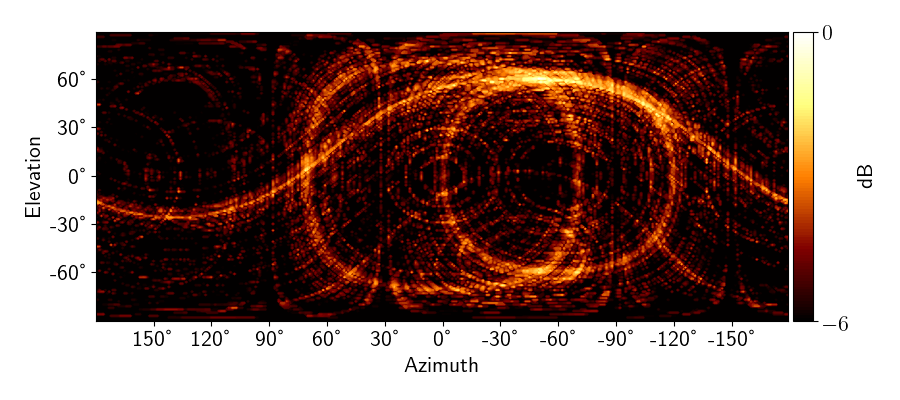
\includegraphics[width=0.8\textwidth]{Figures/Ind4mic1srcResNeg10LowDyn.png}
%\end{subfigure}
%\vskip \baselineskip
%\begin{subfigure}[b]{0.96\textwidth}
%    \centering
%    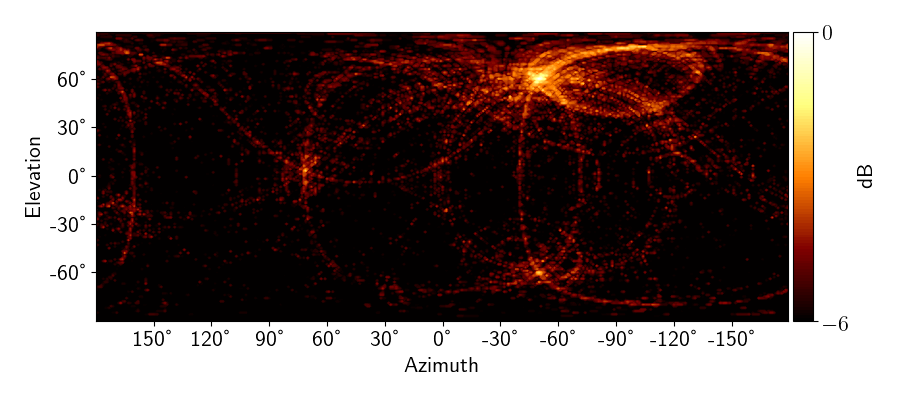
\includegraphics[width=0.8\textwidth]{Figures/Dep4mic1srcResNeg10LowDyn.png}
%\end{subfigure}
%\caption{Figures depict from SRP-PHAT localization results with SNR = -10dB, for independent microphone pairs (top), and for all  microphone pairs (bottom)}
%\label{fig:4mic1srcRedun}
%\end{figure}
%\subsubsection{Simulations}
%Two identical sound sources are placed in the far field. A tetrahedral array with equal spacing between microphones of 1 meter is receiving the two sources. The sound received at the sources are 3 seconds of two different pink noises with respective DOA $\tetha_{1}=120\degree$, $\phi_{1}=40\degree $ and $\tetha_{2}=150\degree $ , $\phi_{2}=75\degree $. Waves are propagating in free field where no reflections and no noise is added to the microphones. The SRP maps are computed and displayed in the figure \ref{fig:coherent2pinknoise}. Source 2 is placed at a problematic angle for the tetrahedral array, detection errors are discussed in section \ref{sec:detection}. Error probability increases as the source DOA approach the angle of the axis drawn by pairs of microphones (end-side).
%\begin{figure}[H]
%    \centering
%    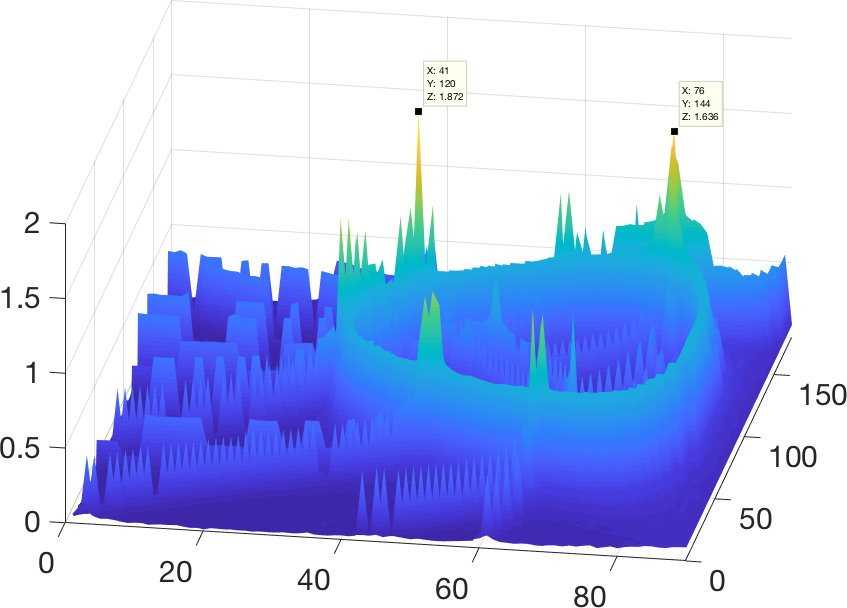
\includegraphics[width=1\textwidth]{Figures/2pinknoisesrpphat.png}
%    \caption{SRP-PHAT simulation with 2 sound sources localized using a tetrahedral array}
%    \label{fig:coherent2pinknoise}
%\end{figure}
%\subsubsection{Localization errors} \label{sec:detection}
%Two pairs of microphones are considered, the axes drawn by the two pairs is plotted (extended) in figure \ref{fig:locerrortetra}. The two axes form respective angles of $45\degree$ and $60\degree$ with the horizontal axis. Plane waves with DOA between $45\degree$ and $60\degree$ will cross the two pairs of microphones at an angle close to the respective end-sides of the pairs. As shown in figure \ref{fig:errorsimulation1} maximum errors arise in the simulation for DOA contained in between $45\degree$ and $60\degree$. For a tetrahedral array, this can be seen as the 3d space created by extending the arms connecting the microphones. 
%\begin{figure}[H]
%    \centering
%    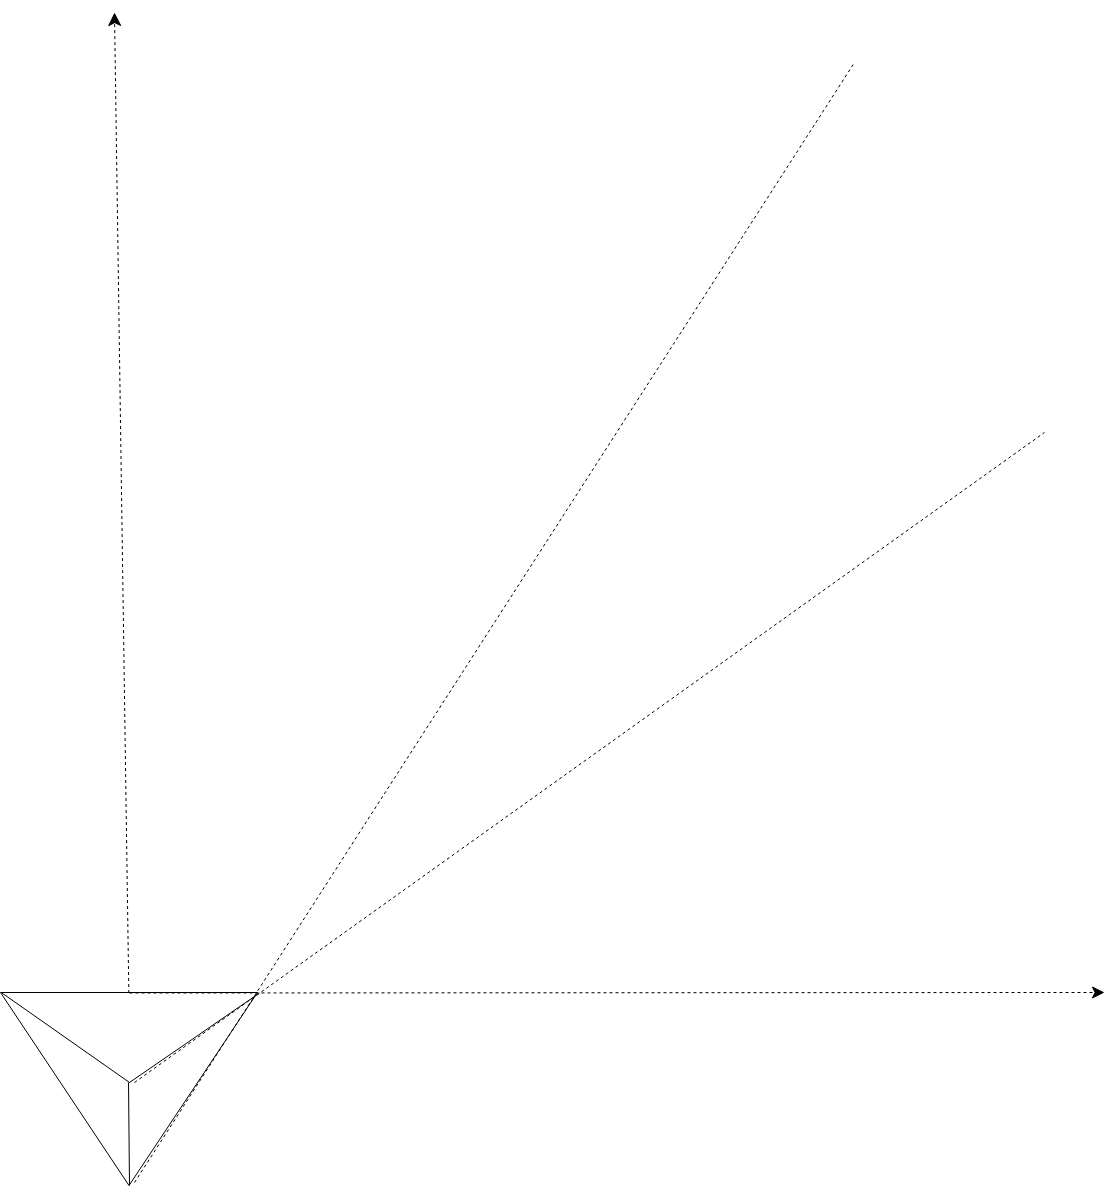
\includegraphics[width=0.9\textwidth]{Figures/locerrors.png}
%    \caption{Axis drawn by 2 pairs of microphones}
%    \label{fig:locerrortetra}
%\end{figure}
%\begin{figure}[H]
%    \centering
%    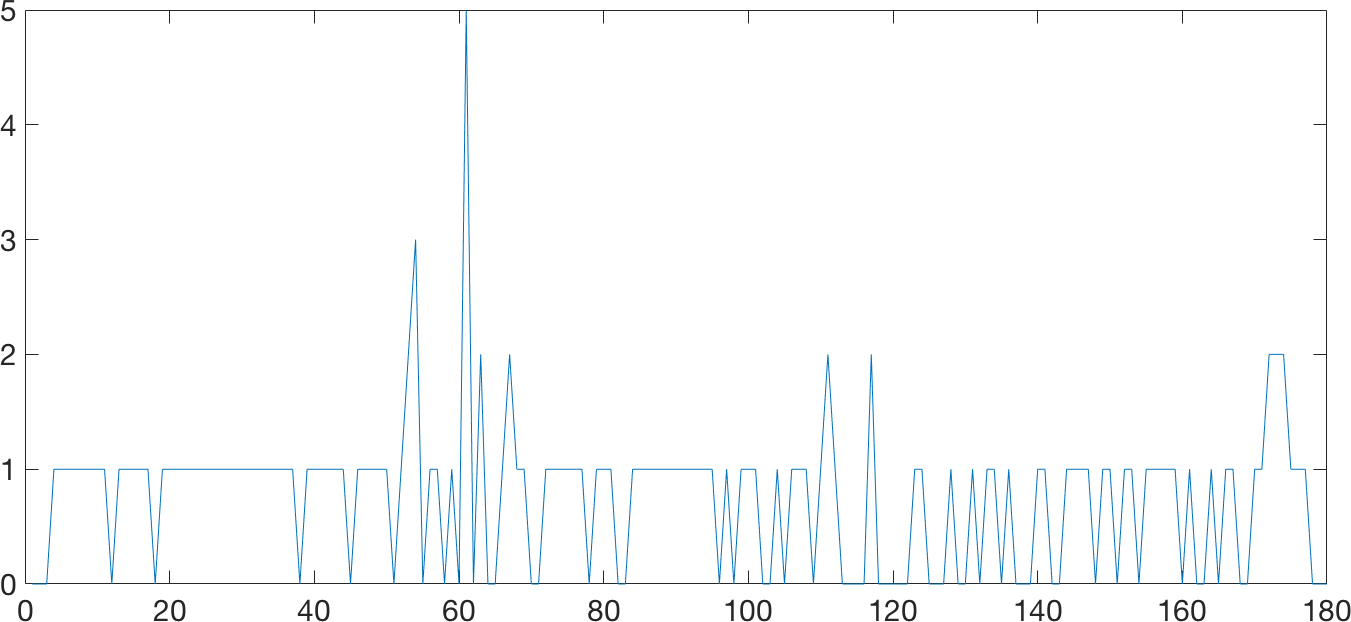
\includegraphics[width=0.9\textwidth]{Figures/errorphinointerpolationandrounding.png}
%    \caption{Simulation errors with no interpolation}
%    \label{fig:errorsimulation1}
%\end{figure}
%\subsubsection{Temperature and noise}
%Temperature is a major parameter of the algorithm and it affects the speed of sound in air and ultimately the propagation delay in the array.
%\subsubsection{SRP vs SRP PHAT}
%An experiment is design to test our implementations of SRP and SRP PHAT. A prototype tetrahedral microphone array is placed outside, the ideal free field condition are not holding since ground effect and reflections from the nearby buildings will affect the sound waves received by the array. The SNR cannot be controlled and is found to be, 